%-----------------------------------------------------------------------------80
% CONTENT
%-----------------------------------------------------------------------------80

\subsection{Proceso de compilación}

\begin{frame}[fragile]{Proceso de compilación}
  \begin{itemize}[<+(1)->]
  \item  El proceso de compilación se puede resumir en dos pasos
  \hspace{1cm} \item [-] Compilación
  \hspace{1cm} \item [-] Enlazado

  \item El proceso de compilación en fortran posee la siguiente sintaxis:
   \begin{mintedbash} 
    fcomp [options] file1 [file2] [...] [fileN]
   \end{mintedbash}
  \item [-] fcomp $\Rightarrow$ denota el comando para llamar al compilador. (gfortran, ifort, ...)
  \item [-] options $\Rightarrow$ opciones que permite el compilador. (-o, -f, -c, ...)
  \item [-] file $\Rightarrow$ denota el archivo con su respectiva extensión (.f90, .f95, .o, ...)    
  \item Finalmente se obtiene un producto final.
\end{itemize}
\end{frame}
  

\begin{frame}[fragile]{Compilación}
\textbf{Compilador}
  \begin{itemize}[<+(1)->]
  \item Programa  escrito en un lenguaje de programación, que a su vez, traduce y genera otro programa
en otro lenguaje de programación (código máquina), ambos equivalentes.
  \item En principio, al usar un compilador, se busca traducir y simplificar un lenguaje de mayor complejidad a uno mucho más cotidiano y manejable en términos informáticos.
 \end{itemize}
\end{frame}


\begin{frame}[fragile]{Compilación}

  \begin{figure}
    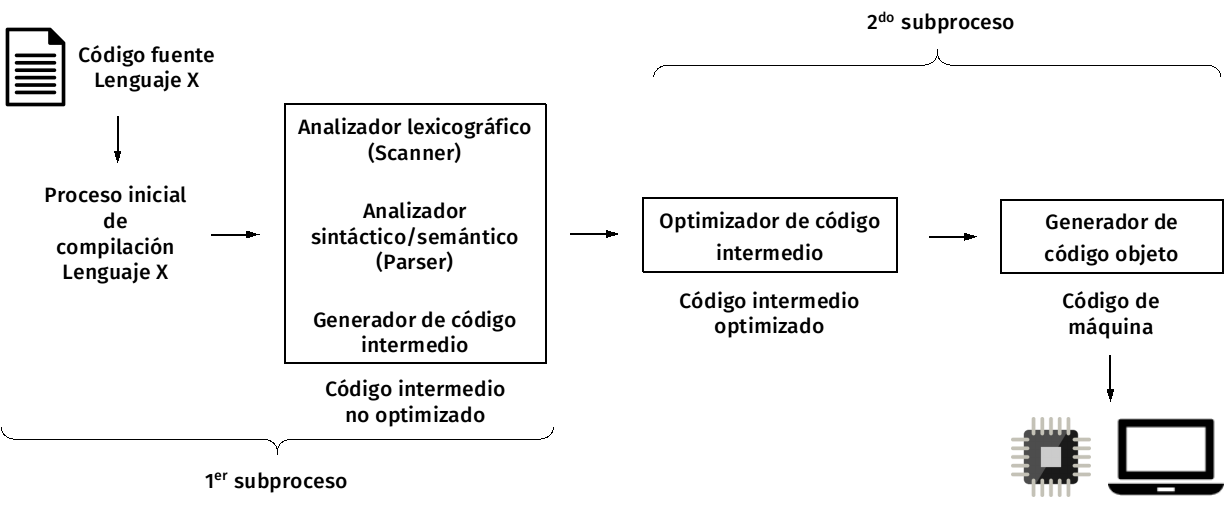
\includegraphics[width=1\textwidth]{./resources/compilation_op.png}
    \caption{Diagrama de bloques del proceso de compilación}
   \end{figure}
\end{frame}